\begin{figure*}
    \centering
    \begin{subfigure}{\textwidth}
    \includegraphics[width=\linewidth,trim={0 13cm 0 0},clip]{binder/binder/teeplots/adaptive-evolution-rate.ipynb/col=components+errorbar=ci+hue=treatment+kind=line+post=plt-xlim-0-600+row=mutation+viz=relplot+x=generation+y=has-task+ext=.pdf}
% \includegraphics[width=\linewidth,trim={0 0 0 24cm},clip]{binder/binder/teeplots/adaptive-evolution-rate.ipynb/col=components+errorbar=ci+hue=treatment+kind=line+post=plt-xlim-0-600+row=mutation+viz=relplot+x=generation+y=has-task+ext=.pdf}
    \caption{\footnotesize including directly-facilitated adaptive variation from slip duplication (tasks gained directly through slip duplication); (blue: long-ancestor; purple: baseline treatment; orange: slip-duplicate treatment)}
    \label{fig:adaptive-evolution-rate:direct}
    \end{subfigure}

%    \begin{subfigure}{\textwidth}
%\includegraphics[width=\linewidth,trim={0 0 0 13cm},clip]{binder/binder/teeplots/adaptive-evolution-rate-nodirect.ipynb/col=components+errorbar=ci+hue=treatment+kind=line+post=plt-xlim-0-600+row=mutation+viz=relplot+x=generation+y=has-task+ext=.pdf}
%    \caption{\footnotesize excluding directly-facilitated adpative variation from slip duplication (only instances where tasks did not arise as an immediate consequence of slip duplication); (brown: long-ancestor; purple: baseline treatment; red: slip-duplicate treatment)}
%    \label{fig:adaptive-evolution-rate:nodirect}
%    \end{subfigure}
    \caption{
        \textbf{Rate of adaptive evolution across a spectrum of task complexities.}
        \footnotesize
        Simple tasks (leftmost panels) require only one logic gate component.
        More complex tasks (rightmost panels) require up to five logic gate components.
        Slip-duplication treatment facilitates significantly faster adaptive evolution than long-genome treatment for more complex tasks, requiring 4 or 5 components (top panel).
        Without instances where tasks were acquired directly through slip duplicaiton, however, no significant difference is detected between the adaptive rates of long-genome and slip-duplication treatments for these more complex tasks (bottom panel).
        Error bands give 95\% CI, bootstrapped over 30 replicates per treatment.
    }
    \label{fig:adaptive-evolution-rate}
\end{figure*}
